\newcommand{\qlogo}[1]{\raisebox{-.25\height}{
\includegraphics[width=#1]{logo}}?}

\newenvironment{planslide}[2]{%
\begin{frame}
\frametitle{#2}

\large 

\begin{tabular}{l c l }

\qlogo{.7cm} &\ & \textcolor{#1}{Motivation and background for Cedille} \\ \\


$\vdash \textit{\textcolor{red}{C}e\textcolor{red}{D}i\textcolor{red}{L}l\textcolor{red}{E}}$ &\ & \textcolor{#1}{Syntax and semantics}\\ \\

\texttt{cedille} &\ & \textcolor{#1}{Tooling: emacs frontend $\leftrightarrow$ backend} \\ \\

$\leadsto\ \texttt{cedille}_{\texttt{core}}$ & \ & \textcolor{#1}{Elaboration to Cedille Core} \\ \\

\texttt{c d ll} &\ & \textcolor{#1}{Spine-local type inference} \\ \\ 

%\begin{tikzpicture}[
%  decoration={
%    reverse path,
%    text effects along path,
%    text={cedille cedille cedille cedille cedille cedille cedille cedille cedille cedille cedille cedille cedille cedille
%      cedille cedille cedille cedille cedille cedille cedille cedille cedille.},
%    text effects/.cd,
%      text along path,
%      character count=\i, character total=\n,
%      characters={scale=1-\i/\n}
%    }
%]
%\draw [decorate] (0,0) 
%    \foreach \i [evaluate={\r=(\i/2400)^2;}] in {0,7,...,2380}{ -- (\i:\r)}; 
%\end{tikzpicture}

\raisebox{-.8\height}{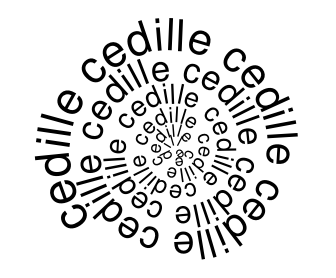
\includegraphics[width=2cm]{cedillespiral}} &\ & 

\textcolor{#1}{Future directions}


\end{tabular}

\end{frame}
}

